\documentclass{article}

% Language setting
% Replace `english' with e.g. `spanish' to change the document language
\usepackage[english]{babel}

% Set page size and margins
% Replace `letterpaper' with `a4paper' for UK/EU standard size
\usepackage[letterpaper,top=2cm,bottom=2cm,left=3cm,right=3cm,marginparwidth=1.75cm]{geometry}

% Useful packages
\usepackage{amsmath}
\usepackage{graphicx}
\usepackage[colorlinks=true, allcolors=blue]{hyperref}
\usepackage{bm}
\usepackage{tikz}
\usetikzlibrary{fit, positioning}

\usepackage{cleveref}
\crefname{figure}{fig.}{fig.}
\Crefname{figure}{Fig.}{Fig.}
\crefname{equation}{eq.}{eq.}
\Crefname{equation}{Eq.}{Eq.}

\usepackage[color=magenta]{todonotes}



\title{Composition of Movement Primitives}
% \author{Andrea Pierré}

\begin{document}
\maketitle

% \begin{abstract}
% Your abstract.
% \end{abstract}

\tableofcontents

\section{ProMPs}
\subsection{Recap}
From \citep{paraschos_probabilistic_2013, paraschos_using_2018}:
\begin{itemize}
    \item $q_t$: joint angle over time
    \item $\dot{q}_t$: joint velocity over time
    \item $\bm{\tau} = \{q_t\}_{t=0\dots T}$: trajectory
    \item $\bm{w}$: weight vector of a single trajectory $[n \times 1]$
    \item $\phi_t$: basis function
    \item $n$: number of basis functions
    \item $\bm{\Phi}_t = [\phi_t, \dot{\phi_t}]$: $n \times 2$ dimensional time-dependent basis matrix
    \item $z(t)$: monotonically increasing phase variable
    \item $\bm{\epsilon}_y \sim \mathcal{N}(\bm{0}, \bm{\Sigma}_y)$: zero-mean i.i.d. Gaussian noise
\end{itemize}

\begin{equation}
  \bm{\Phi}_t =
  \begin{bmatrix}
    \phi_1 & \dot{\phi_1}\\
    \vdots & \vdots\\
    \phi_n & \dot{\phi_n}
  \end{bmatrix}
\end{equation}

\begin{gather}
\bm{y}_t = \begin{bmatrix}
       q_t \\[0.3em]
       \dot{q}_t
     \end{bmatrix} = \bm{\Phi}^{\top}_{t}\bm{w} + \bm{\epsilon}_y\\
p(\bm{\tau}|\bm{w}) = \prod_t \mathcal{N}\Big(\bm{y}_t|\bm{\Phi}^{\top}_{t}\bm{w}, \bm{\Sigma}_y \Big)\\
p(\bm{\tau};\bm{\theta}) = \int p(\bm{\tau}|\bm{w}) \cdot p(\bm{w};\bm{\theta}) d\bm{w}
\end{gather}

\subsection{Coupling between joints}

\begin{equation}
p(\bm{y}_t|\bm{w}) = \mathcal{N}\Bigg(
        \begin{bmatrix}
                \bm{y}_{1,t} \\
                \vdots\\
                \bm{y}_{d,t} \\
        \end{bmatrix}
        \Bigg|
        \begin{bmatrix}
                \bm{\Phi}^{\top}_{t} & \cdots & \bm{0} \\
                \vdots &\ddots & \vdots\\
                \bm{0} & \cdots & \bm{\Phi}^{\top}_{t} \\
        \end{bmatrix}
        \bm{w}, \bm{\Sigma}_y
\Bigg) = \mathcal{N}\Big(\bm{y}_t|\bm{\Psi}_t\bm{w},\bm{\Sigma}_y \Big)
\end{equation}

with:
\begin{itemize}
    \item $\bm{w}=[\bm{w}^\top_1, \dots, \bm{w}^\top_n]^\top$: combined weight vector $[n \times n]$
    \item $\bm{\Psi}_t$: block-diagonal basis matrix containing the basis functions and their derivatives for each dimension
    \item $\bm{y}_{i,t} = [q_{i,t}, \dot{q}_{i,t}]^\top$: joint angle and velocity for the $i^{\text{th}}$ joint
\end{itemize}

\subsection{Hierarchical Bayesian Model}

The Hierarchical Bayesian Model used in ProMPs is illustrated in \Cref{fig:HBM}.

\begin{figure}[htbp]
\centering
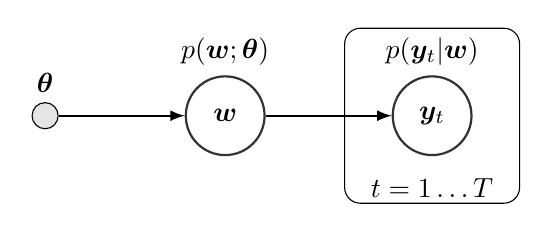
\begin{tikzpicture}
\tikzstyle{main}=[circle, minimum size = 10mm, thick, draw =black!80, node distance = 16mm]
\tikzstyle{connect}=[-latex, thick]
\tikzstyle{box}=[rectangle, draw=black!100]
  \node[circle, draw=black!100, fill = black!10] (theta) [label=above:$\bm{\theta}$] { };
  \node[main] (w) [right=of theta,label=above:$p(\bm{w};\bm{\theta})$] {$\bm{w}$};
  \node[main] (y) [right=of w,label=above:$p(\bm{y}_t|\bm{w})$] {$\bm{y}_t$};
  \path (theta) edge [connect] (w)
		(w) edge [connect] (y);
  \node[rectangle, inner sep=1.5mm, fit= (y),label=below:{$t=1 \dots T$}] (ghost) {};
  \node[rectangle, rounded corners=0.2cm, inner sep=4.4mm,draw=black!100, fit= (y) (ghost)] {};
\end{tikzpicture}
\caption{Hierarchical Bayesian Model used in ProMPs.}
\label{fig:HBM}
\end{figure}

\begin{itemize}
  \item $\bm{\theta} = \{\bm{\mu}_{w}, \bm{\Sigma}_{w}\}$
  \item $p(\bm{w};\bm{\theta}) = \mathcal{N}(\bm{w}|\bm{\mu}_{w}, \bm{\Sigma}_{w})$: prior over the weight vector $\bm{w}$, with parameters $\bm{\theta}$, assumed to be Gaussian
\end{itemize}

\begin{align}
p(\bm{y}_t; \bm{\theta}) &= \int \mathcal{N}\Big(\bm{y}_t|\bm{\Psi}^\top_t \bm{w}, \bm{\Sigma}_y \Big) \cdot p(\bm{w}; \bm{\theta}) \; d\bm{w}\\
&= \int \mathcal{N}\Big(\bm{y}_t|\bm{\Psi}^\top_t \bm{w}, \bm{\Sigma}_y \Big) \cdot \mathcal{N}\Big(\bm{w}|\bm{\mu_w}, \bm{\Sigma_w} \Big) \; d\bm{w}\\
&= \mathcal{N}\Big( \bm{y}_t | \bm{\Psi}^\top_t \bm{\mu_w}, \bm{\Psi}^\top_t \bm{\Sigma_w} \bm{\Psi}_t + \bm{\Sigma}_y \Big)\label{eq:HBM}
\end{align}
See \Cref{proof:HBM} for the proof.


\subsection{Via-Points Modulation}

\begin{itemize}
    \item $\bm{x}_t^\star = [\bm{y}_t^\star, \bm{\Sigma}^\star_t]$: desired observation
    \item $\bm{y}^\star_t$: desired position and velocity vector at time $t$
    \item $\bm{\Sigma}^\star_t$: accuracy of the desired observation
\end{itemize}

Using Bayes rule:
\begin{align}
  p(\bm{w}|\bm{x}_t^\star) &= \frac{p(\bm{x}_t^\star|\bm{w}) \cdot p(\bm{w})}{p(\bm{x}_t^\star)} \\
  p(\bm{w}|\bm{x}_t^\star) &\propto \mathcal{N}\Big( \bm{y}_t^\star | \bm{\Psi}_t^\top\bm{w}, \bm{\Sigma}^\star_t \Big) \cdot \mathcal{N}(\bm{w}|\bm{\mu}_{w}, \bm{\Sigma}_{w})\label{eq:prob-cond-new}
\end{align}

\begin{align}
\bm{\mu_w}^{[new]} &= \bm{\mu_w} + \bm{\Sigma_w}\bm{\Psi}_t \Big(\bm{\Sigma}_y^\star + \bm{\Psi}_t^\top \bm{\Sigma_w}\bm{\Psi}_t \Big)^{-1} (\bm{y}_t^\star - \bm{\Psi}_t^\top \bm{\mu_w})\label{eq:mu-cond-new}\\
\bm{\Sigma_w}^{[new]} &= \bm{\Sigma_w} - \bm{\Sigma_w}\bm{\Psi}_t \Big(\bm{\Sigma}_y^\star +  \bm{\Psi}_t^\top \bm{\Sigma_w}\bm{\Psi}_t \Big)^{-1} \bm{\Psi}_t^\top \bm{\Sigma_w}\label{eq:sigma-cond-new}
\end{align}
See \Cref{proof:conditioning} for the proof.


\subsubsection{Do we actually get the desired mean by applying the conditioning update?}
\begin{equation}
  \bm{\mu}_{\bm{w}|\bm{x}_t^\star} = \bm{\mu_w} + \bm{\Sigma_w}\bm{\Psi}_t \Big(\bm{\Sigma}_t^\star + \bm{\Psi}_t^\top \bm{\Sigma_w}\bm{\Psi}_t \Big)^{-1} (\bm{y}_t^\star - \bm{\Psi}_t^\top \bm{\mu_w})
                          % &\stackrel{?}{=} \bm{y}_t^\star
  \end{equation}
  Let us set the observed covariance $\bm{\Sigma}_t^\star$ to $0$ so as to have perfect accuracy around our observed position.
\begin{align}
  \bm{\mu}_{\bm{w}|\bm{x}_t^\star} &= \bm{\mu_w} + \bm{\Sigma_w}\bm{\Psi}_t \Big( \bm{\Psi}_t^\top \bm{\Sigma_w}\bm{\Psi}_t \Big)^{-1} (\bm{y}_t^\star - \bm{\Psi}_t^\top \bm{\mu_w})\\
                                   &= \bm{\mu_w} + \bm{\Sigma_w}\bm{\Psi}_t \Big( \bm{\Psi}_t^\top \bm{\Sigma_w}\bm{\Psi}_t \Big)^{-1} (\bm{y}_t^\star - \bm{\mu}_{\bm{y}_{t}}) \quad \text{(which does not simplify further)}\\
                                   &\neq \bm{y}_t^\star
  \end{align}

  \subsubsection{Multi via-points}

\begin{figure}[htbp]
  \centering
  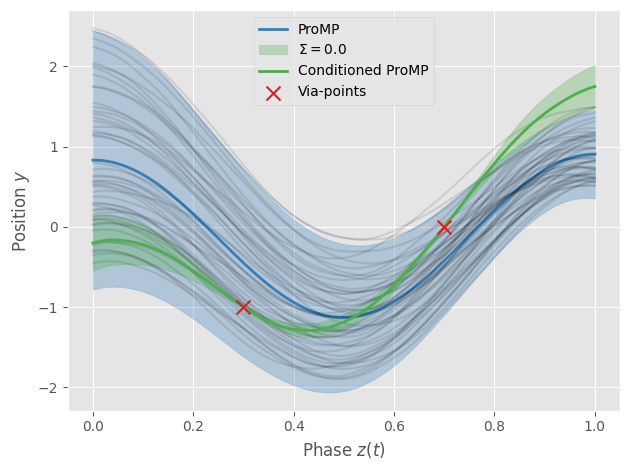
\includegraphics[width=0.5\linewidth]{fig/2-via-points.png}
  \caption{Example of ProMP with two via points.}
  \label{fig:multi-via-pts}
\end{figure}

\todo[inline]{Two points conditional update derivation}


\section{Composition of MPs}
\subsection{Blending}
\subsection{Stitching}



\bibliographystyle{IEEEtranN}
\bibliography{references}


\appendix
\section{Hierarchical Bayesian Model proof}

\begin{proof}[Proof of \Cref{eq:HBM}]\label{proof:HBM}
From \citep{deisenroth2020mathematics}, we have the joint distribution:
\begin{equation}
  p(\bm{\mathrm{x}}_{a}, \bm{\mathrm{x}}_{b}) = \mathcal{N}\Bigg(
  \begin{bmatrix}
    \bm{\mu}_{a} \\
    \bm{\mu}_{b} \\
  \end{bmatrix},
  \begin{bmatrix}
    \bm{\Sigma}_{aa} & \bm{\Sigma}_{ab}  \\
    \bm{\Sigma}_{ba} & \bm{\Sigma}_{bb}
  \end{bmatrix}
  \Bigg)\label{eq:joint-distrib}
\end{equation}

and the marginal distribution $p(\bm{\mathrm{x}}_{a})$ of a joint Gaussian distribution $p(\bm{\mathrm{x}}_{a}, \bm{\mathrm{x}}_{b})$:
\begin{equation}
  p(\bm{\mathrm{x}}_{a}) = \int p(\bm{\mathrm{x}}_{a}, \bm{\mathrm{x}}_{b}) d \bm{\mathrm{x}}_{b} = \mathcal{N}( \bm{\mathrm{x}}_{a} | \bm{\mu}_{a}, \bm{\Sigma}_{aa})
\end{equation}

Since $\bm{y}_t$ and $\bm{w}$ are jointly Gaussian, we have:
\begin{equation}
  \begin{bmatrix}
    \bm{y}_t \\
    \bm{w}
  \end{bmatrix} \sim \mathcal{N}\Bigg(
  \begin{bmatrix}
    \bm{\mu}_{\bm{y}_{t}} \\
    \bm{\mu_w} \\
  \end{bmatrix},
  \begin{bmatrix}
    \mathrm{Cov}[\bm{y}_t, \bm{y}_t] & \mathrm{Cov}[\bm{y}_t, \bm{w}]  \\
    \mathrm{Cov}[\bm{w}, \bm{y}_t] & \mathrm{Cov}[\bm{w}, \bm{w}]
  \end{bmatrix}
  \Bigg)
\end{equation}
\begin{align}
  \bm{\mu}_{\bm{y}_{t}} &= \E[\bm{y}_{t}]\\
                        &= \E[\bm{\Psi}^\top_t \bm{w} + \bm{\epsilon}_y]\\
                        &= \bm{\Psi}^\top_t \E[\bm{w}] + \E[\bm{\epsilon}_y]\\
                        &= \bm{\Psi}^\top_t \bm{\mu_w} + 0\\
                        &= \bm{\Psi}^\top_t \bm{\mu_w}
\end{align}
\begin{align}
  \mathrm{Cov}[\bm{y}_t, \bm{y}_t] &= \mathrm{Cov}[\bm{\Psi}^\top_t \bm{w} + \bm{\epsilon}_y]\\
  &= \mathrm{Cov}[\bm{\Psi}^\top_t \bm{w}] + \mathrm{Cov}[\bm{\epsilon}_y]\\
  &= \bm{\Psi}^\top_t\mathrm{Cov}[\bm{w}]\bm{\Psi}_t + \bm{\Sigma}_{y}\\
    &= \bm{\Psi}^\top_t\bm{\Sigma_{w}}\bm{\Psi}_t + \bm{\Sigma}_{y}\label{eq:cov_y_y}
\end{align}

\begin{equation}
  \begin{bmatrix}
    \bm{y}_t \\
    \bm{w}
  \end{bmatrix} \sim \mathcal{N}\Bigg(
  \begin{bmatrix}
    \bm{\Psi}^\top_t \bm{\mu_w} \\
    \bm{\mu_w} \\
  \end{bmatrix},
  \begin{bmatrix}
    \bm{\Psi}^\top_t \bm{\Sigma_w} \bm{\Psi}_t + \bm{\Sigma}_y & \bm{\Psi}^\top_t \bm{\Sigma_w}  \\
    \bm{\Sigma_w} \bm{\Psi}_t & \bm{\Sigma_w}
  \end{bmatrix}
  \Bigg)
\end{equation}
\begin{equation}
p(\bm{y}_t; \bm{\theta}) = \mathcal{N}\Big( \bm{y}_t | \bm{\Psi}^\top_t \bm{\mu_w}, \bm{\Psi}^\top_t \bm{\Sigma_w} \bm{\Psi}_t + \bm{\Sigma}_y \Big)
\end{equation}

\end{proof}

\section{Via-Points conditioning proof}

\begin{proof}[Proof of \Cref{eq:mu-cond-new} and \Cref{eq:sigma-cond-new}]\label{proof:conditioning}
  With the joint distribution $p(\bm{\mathrm{x}}_{a}, \bm{\mathrm{x}}_{b})$ in \Cref{eq:joint-distrib}, and from \citep{bishop2024learning}, the parameters of a conditional multivariate Gaussian $p(\bm{\mathrm{x}}_{a}|\bm{\mathrm{x}}_{b}) = \mathcal{N}\big( \bm{\mu}_{a|b}, \bm{\Sigma}_{a|b} \big)$ are the following:
\begin{align}
  \bm{\mu}_{a|b} &= \bm{\mu}_{a} + \bm{\Sigma}_{ab}\bm{\Sigma}_{bb}^{-1}(\bm{\mathrm{x}}_{b} - \bm{\mu}_{b})\label{eq:cond-multi-gauss-mu}\\
  \bm{\Sigma}_{a|b} &= \bm{\Sigma}_{aa} - \bm{\Sigma}_{ab}\bm{\Sigma}_{bb}^{-1}\bm{\Sigma}_{ba}\label{eq:cond-multi-gauss-sigma}
\end{align}

We want the posterior $p(\bm{w}|\bm{x}_t^\star)$, knowing the likelihood $\bm{x}_t^\star|\bm{w} \sim \mathcal{N}\Big( \bm{y}_t^\star | \bm{\Psi}_t^\top\bm{w}, \bm{\Sigma}^\star_t \Big)$, and the prior $\bm{w} \sim \mathcal{N}(\bm{w}|\bm{\mu}_{w}, \bm{\Sigma}_{w})$.

\begin{equation}
  \begin{bmatrix}
    \bm{w} \\
    \bm{x}_t^{\star}
  \end{bmatrix} \sim \mathcal{N}\Bigg(
  \begin{bmatrix}
    \bm{\mu_w} \\
    \bm{\Psi}^\top_t \bm{\mu_w}\\
  \end{bmatrix},
  \begin{bmatrix}
    \mathrm{Cov}[\bm{w}, \bm{w}] &  \mathrm{Cov}[\bm{w}, \bm{x}_t^{\star}] \\
    \mathrm{Cov}[\bm{x}_t^{\star}, \bm{w}] & \mathrm{Cov}[\bm{x}_t^{\star}, \bm{x}_t^{\star}]
  \end{bmatrix}
  \Bigg)
\end{equation}

$\mathrm{Cov}[\bm{x}_t^{\star}, \bm{x}_t^{\star}]$ follows from \Cref{eq:cov_y_y}.

\begin{align}
  \mathrm{Cov}[\bm{w}, \bm{x}_t^{\star}] &= \mathrm{Cov}[\bm{w}, \bm{\Psi}^\top_t\bm{w} + \bm{\epsilon}_y]\\
                                         &= \mathrm{Cov}[\bm{w}, \bm{\Psi}^\top_t\bm{w}] & ( \mathrm{Cov}[\bm{w}, \bm{\epsilon_y}] = 0 \text{ since } \bm{\epsilon_y} \text{ is independent of } \bm{w})\\
                                         &= \E[(\bm{w} - \bm{\mu_{w}})(\bm{\Psi}^\top_t\bm{w} - \bm{\Psi}^\top_t\bm{\mu_{w}})^{\top}]\\
                                         &= \E[(\bm{w} - \bm{\mu_{w}})(\bm{w} - \bm{\mu_{w}})^{\top}\bm{\Psi}_t]\\
                                         &= \mathrm{Cov}[\bm{w}, \bm{w}] \cdot \bm{\Psi}_t\\
                                         &= \bm{\Sigma_{w}} \bm{\Psi}_t
\end{align}

\begin{equation}
  \begin{bmatrix}
    \bm{w} \\
    \bm{x}_t^{\star}
  \end{bmatrix} \sim \mathcal{N}\Bigg(
  \begin{bmatrix}
    \bm{\mu_w} \\
    \bm{\Psi}^\top_t \bm{\mu_w}\\
  \end{bmatrix},
  \begin{bmatrix}
     \bm{\Sigma_w} & \bm{\Sigma_{w}} \bm{\Psi}_t  \\
    \bm{\Psi}^\top_t\bm{\Sigma_w} & \bm{\Psi}^\top_t \bm{\Sigma_w} \bm{\Psi}_t + \bm{\Sigma}^\star_t
  \end{bmatrix}
  \Bigg)
\end{equation}

Using \Cref{eq:cond-multi-gauss-mu} we get:
\begin{equation}
\bm{\mu}_{\bm{w}|\bm{x}_t^\star} = \bm{\mu_w} + \bm{\Sigma_w}\bm{\Psi}_t \Big(\bm{\Sigma}_t^\star + \bm{\Psi}_t^\top \bm{\Sigma_w}\bm{\Psi}_t \Big)^{-1} (\bm{y}_t^\star - \bm{\Psi}_t^\top \bm{\mu_w})
\end{equation}

Using \Cref{eq:cond-multi-gauss-sigma} we get:
\begin{equation}
\bm{\Sigma}_{\bm{w}|\bm{x}_t^\star} = \bm{\Sigma_w} - \bm{\Sigma_w}\bm{\Psi}_t \Big(\bm{\Sigma}_t^\star +  \bm{\Psi}_t^\top \bm{\Sigma_w}\bm{\Psi}_t \Big)^{-1} \bm{\Psi}_t^\top \bm{\Sigma_w}
\end{equation}
\end{proof}


\end{document}
